\begin{frame}[label=Torricelli]
  \frametitle{Torricelli}
    Dato il grafico \textit{distanza-tempo} di un punto che si muove, diciamo
    con velocità \textit{v} al tempo \textit{t}, 
    \begin{center}
        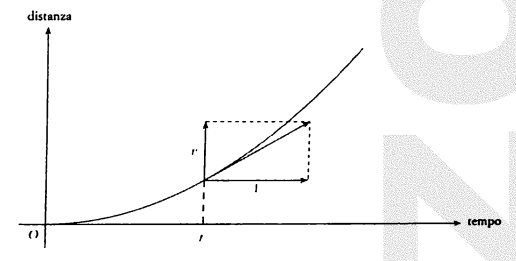
\includegraphics[scale=.4]{distanza-tempo.png}
    \end{center}
    il \alert{coefficiente angolare} misura l'inclinazione della tangente al tempo \textit{t}.
    La velocità è il coefficiente angolare della curva nel grafico distanza-tempo)
    \textit{(Torricelli 1640)}
  \begin{block}{TFC secondo Torricelli}
    \begin{itemize}
        \item La distanza è l'area della velocità (in relazione al tempo)
        \item La velocità è il coefficiente angolare della tangente alla distanza (in relazione al tempo)
    \end{itemize}
  \end{block}  
\end{frame}